\section{Алгоритмы управления лифтами}

	Алгоритм работы системы управления состоит из основного алгоритма, алгоритма подпрограмм,
		реализующих различные режимы работы системы управления (ревизии, деблокировки,
		управления из машинного помещения, нормальной работы, пожарной опасности),
		и алгоритмов дополнительных подпрограмм, реализующих типовые действия,
		производимые в режиме нормальной работы (движение лифта по приказу, остановка кабины на этаже).Алгоритм работы системы управления представлен на рисунке \ref{dk3}.
        
        \begin{figure}[h]
				\centering
				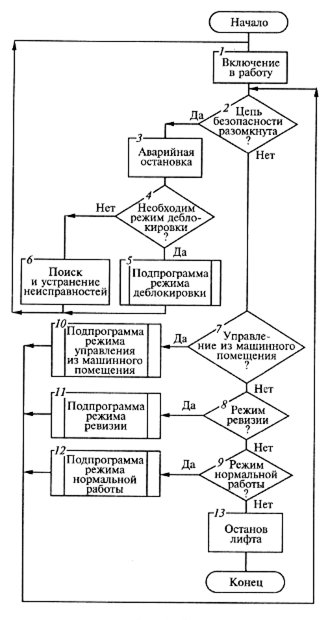
\includegraphics[width=80mm]{src/pictures/algoritm_raboti_sistemi_upravlenia.jpg}
				\caption{Алгоритм работы системы управления}\label{dk3}
        \end{figure}
		% Рис. 3 - Алгоритм работы системы управления
        
    Алгоритм начинается с включения лифта и работу (блок 1), после чего начинается постоянный контроль цепи безопасности (2). Если        цепь разомкнута, происходит аварийная остановка лифта (3). В зависимости от причины аварийной остановки применяется режим        деблокировки (5), если кабина лифта установилась на ловители или конечные выключатели, либо производится определение и            устранение другого рода сбоя в системе (6). Блоки 7...9 определяют необходимость включения того или иного режима работы          лифта, блоки 10...12 реализуют соответствующие подпрограммы. Программа продолжает свою работу до тех пор, пока не будет          выполнен принудительный останов лифта.
    Схема алгоритма подпрограммы, реализующей режим нормальной работы, приведена на рисунке \ref{dk4}.
    
     \begin{figure}[h]
				\centering
				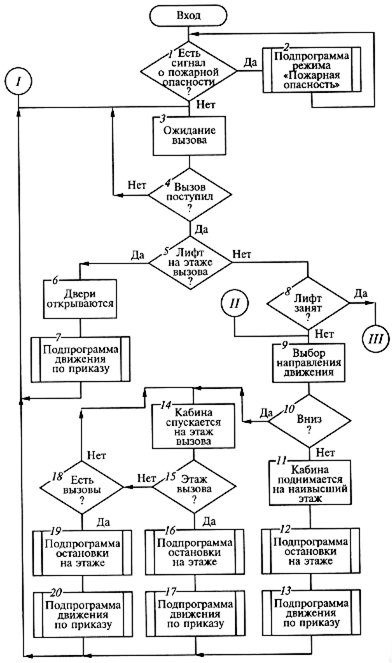
\includegraphics[width=80mm]{src/pictures/algoritm_raboti_podprogrammi.jpg}
				\caption{Алгоритм подпрограммы}\label{dk4}
        \end{figure}
		% Рис. 4 - Схема алгоритма подпрограммы, реализующей режим нормальной работы
        
    В этом режиме производятся контроль пожарной безопасности (2), регистрация и выполнение всех вызовов и приказов, контроль              загруженности кабины. Этот алгоритм составлен с учетом работы системы с собирательным управлением вниз, т.е. выполняются          попутные вызовы при движении кабины вниз (если загрузка менее 90 \% от номинальной), Таким образом, в подпрограмме                реализуются ожидание и регистрация вызова (3, 4), проверка нахождения кабины лифта на этаже вызова (5). В зависимости от          этого осуществляется открытие дверей кабины с последующей работой лифта по приказу (6, 7) или проверяется условие занятости      кабины (8). Если кабина свободна, то блоки 9-20 осуществляют выбор направления движения кабины и в зависимости от этого          после получения приказа выполняются попутные вызовы при движении вниз (если они зарегистрированы) (14-20)или движение          кабины на наивысший из этажей, с которых поступили вызовы, а затем после получения приказа собирательное управление для          движения вниз.

    Если при регистрации вызова кабина занята, вызов выполняется при попутном следовании кабины при условии, что она загружена            менее чем на 90 \% номинальной загрузки. В противном случае, представленном на рисунке \ref{dk5}, ожидают, пока кабина не          освободится или не проследует в попутном направлении, загруженная менее чем на 90 \% (21-29).
    
    \begin{figure}[h]
				\centering
				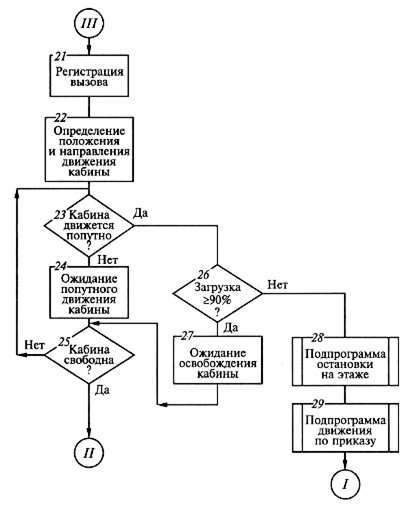
\includegraphics[width=90mm]{src/pictures/image5.jpg}
				\caption{Алгоритм при загрузке кабины более чем на 90 \%}\label{dk5}
    \end{figure}
		% Рис. 5 - Схема работы алгоритма при загрузке кабины более чем на 90 \% номинальной нагрузки

	Система управления лифтом обеспечивает выполнение требований пассажиров
		-- приказы из кабины или запросы с этажей, при этом решая спектр задач,
		которые связаны с определением направления движения в зависимости от взаимного расположения этажа,
		на котором находится кабина лифта, и требуемого этажа, с остановкой кабины на указанном этаже,
		с необходимостью обеспечения безопасного для пассажиров работы лифта,
		а также, связанных с различными режимами работы лифта.

	Первые лифты не были рассчитаны на обработку одновременно нескольких запросов.
		Выполнение запросов производилось только последовательно, каждый последующий запрос
		мог быть произведен только после выполнения предыдущего, даже если вызовы являлись попутными.
		Такой вид управления подъёмником называется последовательным.
		Эта схема управления обеспечивает наиболее простую реализацию схемы управления,
		но пропускная способность лифта при этом невелика. Несмотря на это,
		в некоторых случаях её реализация производится и в настоящее время.
		Например, такая схема управления применяется в грузовых и больничных лифтах,
		а также в пассажирских лифтах для зданий малой и средней этажности.
		Данная схема управления подразумевает, что все запросы пользователей
		фиксируются и исполняются последовательно. В случае поступления одновременных
		запросов команды, которые поступают из кабины лифта являются приоритетными,
		то есть лифт в первую очередь доставляет пассажира на требуемый этаж и только
		после этого перемещается на этаж, с которого был произведен следующий вызов (запрос).

	Следующим этапом развития в данной области стала собирательная схема управления.
		Она получила обширное распространение в жилых зданиях, в которых применяется
		односторонняя собирательная система при движении вниз. Лифт, производящий движение вниз,
		опускаясь на первый этаж, делает остановки в соответствии с запросами от пассажиров с этажей,
		совершая, таким образом, сбор пассажиров. При движении в обратном направлении (снизу-вверх)
		обрабатываются только запросы из кабины, а запросы с этажей игнорируются. Это связано с тем,
		что необходимость в перемещении жителей домов с одного этаж на другой возникает очень редко.
		На аппарате вызова лифта с такой схемой управления располагается только одна кнопка.

	Несколько позже в офисных зданиях и гостиницах стала применяться двусторонняя собирательная система,
		которая обрабатывает запросы с этажей при движении в обоих направлениях. Вызывной аппарат лифтов,
		работающих по данной схеме управления имеет две кнопки – вверх и вниз.
		При вызове производится не только указание необходимого этажа, но и требуемое направления движения.
		Данное усложнение схемы управления обосновывается увеличением пропускной способности лифта.
		Сегодня такая схема управления очень распространена в различных типах зданий.
		В зданиях с большим количеством этажей и интенсивными пассажиропотоками устанавливают
		несколько лифтов (группу лифтов). При этом возникает потребность согласования работы
		лифтов в группе по вызовам, задачами которого являются повышение производительности лифтов,
		уменьшение времени ожидания кабины пассажирами, сокращение (или полное отсутствие)
		количества холостых пробегов и связанное с этим уменьшение износа лифтов и расхода энергии.
		Данные задачи решаются системами группового управления лифтами с применением диспетчеризации.

	Стоит также отметить, что групповое размещение даёт возможность для повышения
		качества лифтового обслуживания при существенной экономии капитальных затрат
		за счет использования общего машинного помещения. Также существенно снижаются
		затраты на проведение технического обслуживания. На протяжении длительного периода
		времени без собирательные, односторонние и полные собирательные схемы управления
		применялись в большинстве зданий, какие-либо принципиально новые решения в системе управления не производились.
		В это время совершенствование схем управления двигалось по пути, как уже говорилось,
		минимизации времени ожидания кабины лифта, что производилось за счет оптимизации схем работы лифтовых групп.
		Известно, что существовали решения на базе нейросетевых технологий.
		Данные решения приносили определенный эффект.

	Один из прогрессивных алгоритмов
		управления группой лифтов был разработан в американской компании Otis Elevator,
		подразумевающий, что каждый пассажир перед посадкой указывает необходимый для него этаж.
		В соответствии с этим система сообщает в какой лифт садиться
		и через какой промежуток времени пребудет кабина. При этом на каждой посадочной площадке
		устанавливается приказная панель, аналогичная той, которая расположена в кабине лифта.
		При оптимизации движении лифтов в качестве целевой функции принимается количество остановок,
		которые делает кабина лифта и данную величину необходимо минимизировать.
		Таким образом, чем меньше кабина де- лает остановок, тем быстрее она возвращается
		на главный посадочный этаж, при этом за счёт меньшего количества попутных остановок
		происходит существенная экономия электроэнергии и сокращение времени кругового рейса кабины лифта.

	Посадка пассажиров близких этажей производится в один лифт с целью минимизации времени поездки
		и уменьшения количества остановок.
		
	Достаточно большое распространение в системах управления группой лифтов получил круговой алгоритм управления.
		Его преимуществами является простота реализации, равномерное распределение нагрузки между лифтами в группе,
		а также обеспечение выполнения требований пассажиров на приемлемом уровне
		при сравнительно не интенсивном пассажиропотоке.
		Основной целью круговой системы при диспетчерском управлении группой лифтов является
		достижение равной загрузки каждого лифта. Вызовы распределяются по мере
		их поступления последовательным образом по отдельным лифтам.
		Вызов 0 назначается к обслуживанию кабиной 0, вызов 1 – кабиной 1, вызов L–кабиной 0,
		вызов L+1 – кабиной 1 и так далее.

	Частным случаем кругового алгоритма представляет собой диспетчерское управление
		при максимальном потоке пассажиров вверх, отличием которого является использовании
		особой стратегии движения. Данная стратегия заключается в том, что,
		если групповой контроллер обнаруживает простаивающий лифт,
		он производит инициализацию вызова на первый этаж для уменьшения времени ожидания будущих пассажиров.

	Алгоритм трех переходов, представленный Ронгом и Хаконеном в 2003 году,
		используется для определения последовательности обслуживания вызовов с этажей.
		Алгоритм разбивает все вызовы на 3 категории:
		\begin{itemize}
			\item[--] вызовы, которые лифт может обслужить без изменения направления движения;
			\item[--] вызовы, которые лифт может обслужить после того, как один раз изменит направление движения;
			\item[--] вызовы, которые лифт может обслужить после того, как дважды изменит направление движения.
		\end{itemize}
	
	Приоритет выполнения вызовов убывают от первой группы к третьей.
	
	В некоторых случаях используют идею зонирования высотных зданий по вертикали,
		которая заключается в разделении здания на несколько прилегающих друг к другу зон
		и каждый из лифтов обрабатывает вызовы с этажей только зоны, назначенной для обслуживания данным лифтом.

	Как правило, разделение здания на зоны с целью оптимизации движения
		лифтов производится в высотных административных зданиях,
		но данная концепция может также применяться и для обычных жилых здания.
		Оптимизация данной стратегии проводится при помощи правильного определения размеров выделяемых зон,
		при этом могут быть учтены такие параметры как численность жильцов на этажах,
		а также некоторые приоритеты обслуживания каких-либо этажей,
		которая определяется на основе набора условий, определяемых отдельно в каждом конкретном случае.

	Также применение идеи зонирования позволяет использовать технические этажи
		для размещения машинных помещений для лифтов, что сокращает потери полезной площади здания.
		Размещение оборудования на технических этажах позволяет уменьшить
		затраты на решение проблемы защиты от шума и вибраций,
		хотя на текущий момент данная потребность не является актуальной,
		так как в настоящее время производители лифтового оборудования выпускают изделия,
		отличающееся достаточно низким уровнем шума.

	В процессе развития алгоритмов управления лифтов в составе группы кроме детерминированных
		классических стратегий появились динамические стратегии автоматизированного управления лифтами.
		В рамках данных стратегий существуют подходы, которые позволяют произвести переход
		от жестких схем управления к гибким, способным подстраиваться к изменениям условий в процессе
		функционирования (изменение интенсивности пассажиропотока или выход из строя лифтов
		в составе лифтовой группы).
	
	Одной из таких является стратегия на основе поиска,
		сущность которой заключается в нахождении оптимального решения при каждом новом возникающем
		событии (например, вызове с этажа), при этом формируется определённая реакция на данное событие.

	Алгоритм поиска производит решение задачи назначения,
		которая заключается в распределении зафиксированных вызовов между лифтами в группе с учётом команд,
		которые произвелись из кабины лифта. Если количество свободных лифтов больше числа произведённых вызовов,
		то алгоритм распределит их в соответствии с определенными критериями.
		В случае, если количество вызовов превышает количество свободных лифтов,
		то из множества заявок будут выделены те, обслуживание которых обеспечит минимум целевой функции,
		например, среднее время ожидания.
		
	Недостатком данной стратегии является статичность в интервале формирования решений,
		что означает тот факт, что новые вызовы, которые поступили после назначения
		не имеют возможности изменить решение системы управления.
		Для нивелирования данного недостатка применяется переопределение управляющего воздействия,
		которое подразумевает корректировку решения согласно с новой текущей ситуации.
		Стоит отметить, что данное решение существенно повышает вычислительную сложность алгоритма.
		По этой причине данный метод целесообразно применять при достаточно высокой плотности
		пассажиропотока и когда другие подходы не дают существенного повышения эффективности.

	Большое количество алгоритмов управления, которые реализуются на базе контроллеров,
		относятся к стратегии, описываемой набором правил в терминах «IF-THEN» логики.
		Такие правила составляются на основе опыта, полученного в процессе функционирования
		системы или сформулированных по результатам соответствующих научных исследований.
		Данный решение, как правило, используется в области искусственного интеллекта,
		но может быть применено также в системах управления лифтовым оборудованием, оснащенной множеством датчиков.

	Использование нечеткой логики может существенность расширить возможности методов,
		основанных на определении правил, и повысить уровень вариативности системы управления,
		увеличивая число степеней свободы путем повышения уровня детализации условия
		в сравнении со стандартной бинарной логикой.

	Наряду с этим имеется возможность решать задачи управления при помощи применения
		генетических алгоритмов, которые подразумевают имитацию процесса эволюции – гены родителя наследуются потомками.

	В системах с применением искусственного интеллекта генетические алгоритмы рассматриваются
		как совокупность отдельных шагов. Для имитации процесса эволюции
		требуется создать множество правил, на основе которых формируются промежуточные решения.

	Из этого множества может быть сформирован алгоритм управления,
		при этом начальный родительский алгоритм-ген может быть сформирован случайным образом.
		Сам же процесс эволюции в этом случае представляет собой «слияние» генов получение
		в итоге гена-потомка – определенного решения.
		Перед «слиянием» производится определение перспективности смешиваемых алгоритмов
		путем проведения экспериментов, направленных на определение эффективности алгоритмов
		и обеспечения взвешенного выбора правил. Таким образом, алгоритмы с каждой итерацией
		будут совершенствоваться, приближаясь к некоторому идеалу и после окончания итераций
		будет получен некоторый усовершенствованный алгоритм управления.

	Один из недостатков генетических алгоритмов заключается в их высокой трудоемкости,
		обусловленная итерационным характером реализации данных алгоритмов.
		Использование для вычисления параллельных структур, таких как, например,
		программируемых логических интегральных схем (ПЛИС),
		снижает влияние данного недостатка. Но более критичным недостатком является тот факт,
		что эффективность алгоритма определяется исходным набором правил,
		если в числе которого нет некоторого правила, то данное правило никогда не появится в порожденных алгоритмах.

	Стоить сделать замечание, что при применении динамических стратегий управления их эффективность
		во многом будет зависеть от числа «степеней свободы», которыми обладает система,
		например, количество лифтов в составе лифтовой группы.
